% vim:syntax=tex

\begin{figure*}[t]
    \centering
\begin{subfigure}[t]{.9\textwidth}
    \centerline{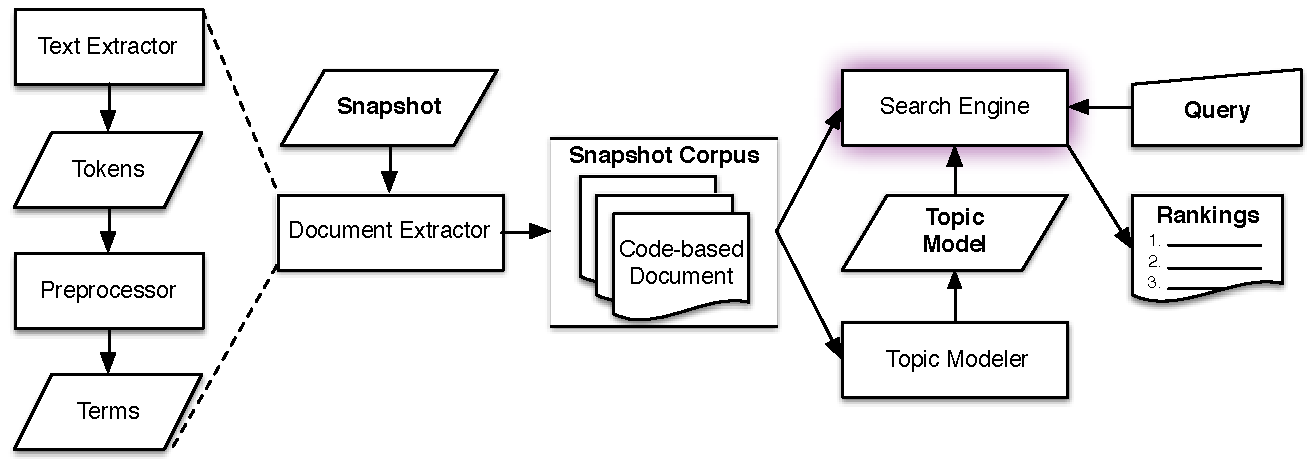
\includegraphics[width=\textwidth]{figures/snapshot-flt}}
    \caption{Topic-modeling-based feature location technique using snapshots}
    \label{fig:snapshot}
\end{subfigure}

\begin{subfigure}[b]{.9\textwidth}
    \centerline{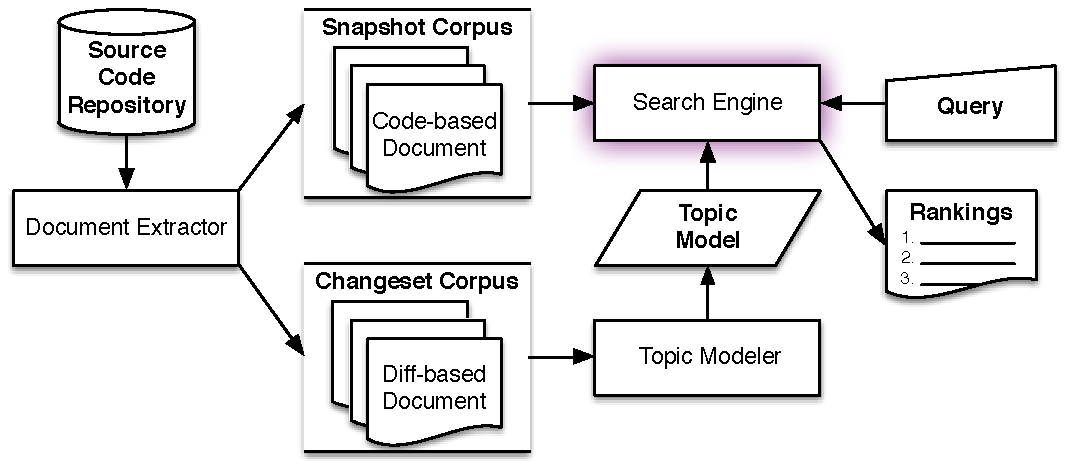
\includegraphics[width=\textwidth]{figures/changeset-flt}}
\caption{Topic-modeling-based feature location technique using changesets}
\label{fig:changeset}
\end{subfigure}

\label{fig:flts}
\caption{Two feature location techniques side-by-side}
\end{figure*}


In this section, we review the standard methodology for document extraction and
retrieval process used by snapshot-based FLTs, as well as related work on topic
modeling and feature location.

\subsection{Document Extraction and Retrieval Process}
\label{sec:snapshot-flt}

We use the following terminology to describe document extraction of a source
code snapshot. A \textit{word} is the basic unit of discrete data in a software
lexicon and is a sequence of letters. A \textit{token} is a sequence of
non-whitespace characters containing one or more words. An \textit{entity} is a
named source element such as a method, and an \textit{identifier} is a token
representing the name of an entity. \textit{Comments} and \textit{literals} are
sequences of tokens delimited by language-specific markers (e.g., /* */ and
quotes). The \textit{document} which corresponds to an entity is a sequence of
words $d = (w_1, \ldots, w_m)$, and a \textit{corpus} is a set of documents
(e.g., methods) $D = (d_1, \ldots, d_n)$.

The left side of Figure~\ref{fig:snapshot} illustrates the document extraction
process. A document extractor takes a source code snapshot as input and produces
a corpus as output. Each document in the corpus contains the words associated
with a source code entity, such as a class or method. The text extractor is the
first part of the document extractor and parses the source code to produce a
token stream for each document. The preprocessor is the second part of the
document extractor. It applies a series of transformations to each token and
produces one or more words from the token. The transformations commonly used
are~\cite{Marcus-etal_2004,Marcus-Menzies_2010,Lawrie-etal_2010}:
\begin{itemize}
    \item {\it Splitting}: separate tokens into constituent words based on
        common coding style conventions (e.g., the use of camel case or
        underscores) and on the presence of non-letters (e.g., punctuation or
        digits)
    \item {\it Normalizing}: replace each upper case letter with the
        corresponding lower case letter
    \item {\it Filtering}: remove common words such as articles (e.g., `an' or
        `the'), programming language keywords, standard library entity names, or
        short words
\end{itemize}

The right side of Figure~\ref{fig:snapshot} illustrates the retrieval process.
The main prerequisite of the retrieval process is to build the search engine.
The search engine is constructed from a topic model trained from a corpus and an
index of that corpus inferred from that model. This means that an index is no
more than each input document's thematic structure (i.e., the document's
inferred topic distribution).

The primary function of the search engine is to rank documents in relation to
the query~\cite{Croft-etal_2010}. First, when using a TM-based approach, the
engine must first infer the thematic structure of the query. This allows for a
pairwise classification of the query to each document in the index and ranks the
documents based on the similarities of their thematic structures.

\subsection{Latent Dirichlet Allocation}

LDA~\cite{Blei-etal_2003} is a generative topic model. LDA models each document
in a corpus of discrete data as a finite mixture over a set of topics and models
each topic as an infinite mixture over a set of topic probabilities. That is,
LDA models each document as a probability distribution indicating the likelihood
that it expresses each topic and models each topic that it infers as a
probability distribution indicating the likelihood of a word from the corpus
being assigned to the topic.

Hoffman et al.~\cite{Hoffman-etal_2010} introduce \textit{online LDA}, an online
version of LDA. Online LDA allows the model to be updated incrementally without
needing to know about the documents prior to model construction. Zhai and
Boyd-Graber~\cite{Zhai-Boyd-Graber_2013} introduce an extension of LDA in which
the model also does not need to know about the corpus vocabulary prior to
training. Teh et al.~\cite{Teh-etal_2006} introduce an LDA counterpart, the
Hierarchical Dirichlet process (HDP), that learns the appropriate number of
topics from the data, rather than needing configuration. Further, Wang et
al.~\cite{Wang-etal_2011} further extend HDP to bring the algorithm online.


\subsection{Feature Location}

Feature location is the act of identifying the source code entity or entities
that implement a feature~\cite{Rajlich-Wilde_2002}. Dit et
al.~\cite{Dit-etal_2013a} provide a taxonomy and survey of feature location in
source code covering the scope of FLTs. They identify 89 works related to
feature location in their systematic literature survey and extract 7 dimensions
for their taxonomy. The primary dimension, type of analysis, can be used for
categorization purposes and consists of four categories: dynamic, static,
historical, and textual. Our methodology uses historical analysis (e.g.,
\cite{Cubranic-etal_2005}) and textual analysis (e.g., \cite{Marcus-etal_2004}).

The most relevant FLTs, by Rao~\cite{Rao-etal_2013,Rao_2013}, are described in
the introduction. Other closely related work involves LSI-based
FLTs~\cite{Marcus-etal_2004,Poshyvanyk-etal_2006,Poshyvanyk-Marcus_2007,Liu-etal_2007,Scanniello-Marcus_2011,Cubranic-etal_2005}
or LDA-based
FLTs~\cite{Lukins-etal_2008,Lukins-etal_2010,Biggers-etal_2014,Bassett-Kraft_2013}.

\subsection{Modeling Software Repositories}

Our work is also not the first to investigate ways to employ topic models on
software repositories. Thomas et al.~\cite{Thomas-etal_2011} present a study on
how topics of a software project evolve over time. They present the \emph{Diff}
model, and closely resembles our work. However, their Diff model is much more
coarse-grained and trains a topic model on changesets between two software
snapshots, not changesets between two commits. Additionally, their goal in using
this model is for modeling the evolution of topics, not for feature location.

\todo{R1: constrast our approach here}
Hindle et al.~\cite{Hindle-etal_2009} present a technique that relates commits
to requirements documents using LDA. They apply LDA to extract topics from issue
reports, requirements documents, and commit messages. Their linking process
relies on LDA inferencing to derive the topics of unseen documents. Hindle et
al.~\cite{Hindle-etal_2014} use a similar approach. Our methodology is based on
the same inferencing concept and creates an index of source code entities from
learned changeset topics.
